%================================================================%
%=============  Modelo de Trabalho de Conclusão de curso ========%
%========================  IFMG =================================% 
% AUTORES:
% prof. Elias J R Freitas =======================================%
% ej-ensino.com.br
%
% baseado no modelo DEPRO-UFOP ==================================%
% estrutura elaborada inicialmente por
% Marcelus Xavier Oliveira  email: marcelusxavier@gmail.com =====%
% Dayanne Gouveia Coelho  email: dayagc@gmail.com ===============%

%================================================================%
% Proposta de texto em conformidade com normas da ABNT ----------%
% Modelo em conformidade com 
% Manual de Normalização de Trabalhos Acadêmicos 21/02/2020
% https://www.ifmg.edu.br/portal/ensino/bibliotecas/
% arquivos-bibliotecas/copy_of_ManualdeNormalizaoIFMG2020.pdf
% implementadas pelo projeto abntex2, que pode ser acessado pela %
% página  http://abntex2.googlecode.com/  -----------------------%
%================================================================%

%================================================================%
% Versao abntex2
%======================== Versão 2022/08 ========================%
%================================================================%


\documentclass[12pt, % tamanho da fonte
	%openright,	% capítulos começam em pág ímpar
	oneside, %para impressão apenas em um lado (formato digital).  		  
	% twoside, %para impressão em frente e verso.  
	a4paper,			% tamanho do papel. 
	english,			% Idioma adicional para hifenização
	brazil				% Idioma principal 
	]{packages/abntex2-ifmg}
	
%------------------------------------------------------------
%------------    Estrutura do texto   -----------------------         

% Pacotes Básicos:
%\usepackage{lmodern}			    % Usa a fonte Latin Modern			

\usepackage[T1]{fontenc}		  % Selecao de codigos de fonte.
\usepackage[utf8]{inputenc}		% Codificacao do documento (conversão automática dos acentos)
\usepackage{mathptmx,helvet,courier}

%\usepackage{pslatex}                % Usa a fonte Times New Roman
\usepackage{lastpage}			    % Usado pela Ficha catalográfica
\usepackage{indentfirst}		  % Indenta o primeiro parágrafo de cada seção.
\usepackage[table]{xcolor}
\usepackage{color}				    % Controle das cores
\usepackage{graphicx}			    % Inclusão de gráficos
\usepackage{microtype} 		  	% para melhorias de justificação

\usepackage{tablefootnote} % para colocar footnotes em tabelas e figuras

% Pacotes Extras:
\usepackage[final]{pdfpages}
\usepackage{amsmath,amsthm}   %Símbolos Matemáticos
\usepackage{indentfirst} % Indenta primeiro parágrafo 
\usepackage[portuguese, ruled, linesnumbered,commentsnumbered, algo2e, vlined, lined, boxed, algochapter]{algorithm2e} % 
\usepackage{algorithm}
\usepackage{algpseudocode}


\usepackage{hyperref}
\usepackage{lineno,hyperref}
\usepackage[brazilian,hyperpageref]{backref}	 % Paginas com as citações na bibliograficas

%\usepackage[num]{abntex2cite}	% Citações padrão ABNT númerico
\usepackage[alf,abnt-emphasize=bf,abnt-full-initials=no,abnt-etal-list=5,abnt-etal-text=emph,abnt-repeated-author-omit=yes]{abntex2cite}
%\usepackage[alf,abnt-emphasize=bf,abnt-etal-list=0,abnt-etal-text=emph]{abntex2cite}

% se desejar justificar as referências (pela abnt é alinhado a esquerda)
% \usepackage[alf,abnt-emphasize=bf,bibjustif]{abntex2cite}

\usepackage{float} % para ajustar a posição das imagens

\usepackage{tikzsymbols} %para caracteres emoji
\usepackage{stackengine}
\usepackage{scalerel}
\usepackage{lscape}
\newcommand\dangersign[1][2ex]{%
  \renewcommand\stacktype{L}%
  \scaleto{\stackon[1.3pt]{\color{red}$\triangle$}{\tiny\bfseries !}}{#1}%
}

\usepackage{etoolbox}
%\usepackage[num]{abntex2cite}  % Citações numéricas

\usepackage{lipsum}

%para usar os algoritmos e matematica
\newcommand{\var}{\texttt}

\usepackage{amssymb}
\usepackage{amsmath}



% Defininfo Cores:
\definecolor{blue}{RGB}{25,25,112}
\definecolor{midgray}{gray}{.7}

\makeatletter % informações do PDF
\hypersetup{ % pagebackref=true,
	pdftitle={\@title}, 
	pdfauthor={\@author},
    pdfsubject={\imprimirpreambulo},
	pdfcreator={LaTeX with abnTeX2},
	pdfkeywords={abnt}{latex}{abntex}{abntex2}{trabalho acadêmico}, 
	colorlinks=true,     % false: boxed links; true: colored links
    linkcolor=black,          	% color of internal links
    citecolor=black,        		% color of links to bibliography
    filecolor=magenta,      	% color of file links
    urlcolor=black,
	bookmarksdepth=4 }
\makeatother
 

% -------------------------------------------- 
% Espaçamentos entre linhas e parágrafos 
\setlength{\parindent}{1.3cm} % O tamanho do parágrafo

% Controle do espaçamento entre um parágrafo e outro:
\setlength{\parskip}{0.2cm}  % tente também \onelineskip

% Definição de ambientes matemáticos em português 
\newtheorem{teorema}{Teorema}[chapter]
\newtheorem{axioma}{Axioma}[chapter]
\newtheorem{corolario}{Corolário}[chapter]
\newtheorem{lema}{Lema}[chapter]
\newtheorem{proposicao}{Proposição}[chapter]
\newtheorem{definicao}{Definição}[chapter]
\newtheorem{exemplo}{Exemplo}[chapter]
\newtheorem{observacao}{Observação}[chapter]

% Novos Comandos
\usepackage{tgtermes}
\renewcommand{\ABNTEXchapterfont}{\rmfamily\bfseries}


\providecommand{\imprimirnomemes}{}
\newcommand{\nomemes}[1]{\renewcommand{\imprimirnomemes}{#1}}

% Variáveis adicionais
\providecommand{\imprimirautorcite}{}
\newcommand{\autorcite}[1]{\renewcommand{\imprimirautorcite}{#1}} 

\providecommand{\imprimirsigla}{}
\newcommand{\sigla}[1]{\renewcommand{\imprimirsigla}{#1}}

\providecommand{\imprimircampus}{}
\newcommand{\campus}[1]{\renewcommand{\imprimircampus}{#1}}

\providecommand{\imprimiruf}{}
\newcommand{\uf}[1]{\renewcommand{\imprimiruf}{#1}}
\providecommand{\imprimircurso}{}
\newcommand{\curso}[1]{\renewcommand{\imprimircurso}{#1}}
\providecommand{\imprimirinstituto}{}
\newcommand{\instituto}[1]{\renewcommand{\imprimirinstituto}{#1}}
\providecommand{\imprimirdepartamento}{}
\newcommand{\departamento}[1]{\renewcommand{\imprimirdepartamento}{#1}}
\providecommand{\imprimirano}{}
\newcommand{\ano}[1]{\renewcommand{\imprimirano}{#1}}
\providecommand{\imprimirdia}{}
\newcommand{\dia}[1]{\renewcommand{\imprimirdia}{#1}}
\providecommand{\imprimirmes}{}
\newcommand{\mes}[1]{\renewcommand{\imprimirmes}{#1}}
\providecommand{\imprimirgrau}{}
\newcommand{\grau}[1]{\renewcommand{\imprimirgrau}{#1}}
\providecommand{\imprimirexaminadorum}{}
\newcommand{\examinadorum}[1]{
    \renewcommand{\imprimirexaminadorum}{#1}}
\providecommand{\imprimirexaminadordois}{}
\newcommand{\examinadordois}[1]{
    \renewcommand{\imprimirexaminadordois}{#1}}
\providecommand{\imprimirexaminadortres}{}
\newcommand{\examinadortres}[1]{
    \renewcommand{\imprimirexaminadortres}{#1}}
\providecommand{\imprimirexaminadorquatro}{}
\newcommand{\examinadorquatro}[1]{
    \renewcommand{\imprimirexaminadorquatro}{#1}}
\providecommand{\imprimirttorientador}{}
\newcommand{\ttorientador}[1]{
    \renewcommand{\imprimirttorientador}{#1}} 
\providecommand{\imprimirttcoorientador}{}
\newcommand{\ttcoorientador}[1]{
    \renewcommand{\imprimirttcoorientador}{#1}}
\providecommand{\imprimirttexaminadorum}{}
\newcommand{\ttexaminadorum}[1]{
    \renewcommand{\imprimirttexaminadorum}{#1}}
\providecommand{\imprimirttexaminadordois}{}
\newcommand{\ttexaminadordois}[1]{\renewcommand{
        \imprimirttexaminadordois}{#1}}
\providecommand{\imprimirttexaminadortres}{}
\newcommand{\ttexaminadortres}[1]{
    \renewcommand{\imprimirttexaminadortres}{#1}}
\providecommand{\imprimirttexaminadorquatro}{}
\newcommand{\ttexaminadorquatro}[1]{
    \renewcommand{\imprimirttexaminadorquatro}{#1}}


% Cria o comando \subtitulo. A norma define que o TITULO deve ser em caixa alta
% negrito, mas o subtitulo deve ser em caixa baixa.
\providecommand{\imprimirsubtitulo}{}
\newcommand{\subtitulo}[1]{\renewcommand{\imprimirsubtitulo}{#1}}

%----------------------------------------------------
\renewcommand{\imprimircapa}{  % Capa 
\begin{capa}
%\begin{center}\includegraphics[scale=1]{Figuras/ifmg.png}\end{center}
\begin{center}{
             \large \MakeTextUppercase{\imprimirinstituicao} - \MakeTextUppercase{\imprimirinstituto} \\
              %\imprimirdepartamento \\
              \MakeTextUppercase{\imprimircurso} \\
              \vspace{2cm}
			  \large {\imprimirautor} 
			  }\end{center}
\vfill
        \begin{center}
        \MakeTextUppercase{\large \textbf{\imprimirtitulo}}  \\
        \MakeTextLowercase{\textbf{\imprimirsubtitulo}}
				\vspace{2cm}
				%{\large \imprimirautor} 	
				\vfill
        {\large{\imprimirlocal~-~\imprimiruf \\ \imprimirano }}
        \end{center}
\end{capa}   } % Capa

%----------------------------------------------------
\renewcommand{\imprimirfolhaderosto}{% folha de rosto
    \begin{center}
    {{\MakeTextUppercase \imprimirautor}}  \\
		\vfill
		\large {\textbf{\MakeTextUppercase{\imprimirtitulo}}\\
        \MakeTextLowercase{\textbf{\imprimirsubtitulo}}}
    \end{center}
    \vfill 
    \begin{flushright} 
    \parbox{0.6\linewidth}{
		\imprimirtipotrabalho~apresentado ao \imprimirinstituto,~do \imprimirinstituicao,~como parte das exigências do curso de \imprimircurso~para a obtenção do título de \imprimirgrau. \\
		\vfill
		\textbf{\imprimirorientadorRotulo}~\imprimirorientador \\
		\vfill 
		\textbf{\imprimircoorientadorRotulo}~\imprimircoorientador}
   \end{flushright} 
   
	 \vfill
   \begin{center}
   {\large{\imprimirlocal~- \imprimiruf \\ \imprimirano}}
   \end{center} }  % folha de rosto

%----------------------------------------------------


%================================================================================
% Pacotes de citações
%================================================================================

% Configurações do pacote backref
% Texto padrão antes do número das páginas
\renewcommand{\backref}{}
% Define os textos da citação
\addto\captionsbrazil{% portugues-brasil
    % Usado sem a opção hyperpageref de backref
    %\renewcommand{\backrefpagesname}{Citado na(s) p{\'a}gina(s):~}
    \renewcommand*{\backrefalt}[4]{
    	\ifcase #1 %
    		%Nenhuma cita{\c c}{\~a}o no texto.%
    	\or
    		%Citado na p{\'a}gina #2.%
    	\else
    		%Citado #1 vezes nas p{\'a}ginas #2.%
    	\fi}%
}
\addto\captionsenglish{% ingles
    % Usado sem a opção hyperpageref de backref
    \renewcommand{\backrefpagesname}{Cited on page(s):~}
    \renewcommand*{\backrefalt}[4]{
    	\ifcase #1 %
    		No citation.%
    	\or
    		Cited on page #2.%
    	\else
    		Cited #1 times on pages #2.%
    	\fi}%
}
% ---
\makeatletter
\newcommand\thefontsize{Fonte tamanho: \f@size pt}
\makeatother



% para não deixar uma figura sozinha no centro de uma página,
% mas no topo da página.
\makeatletter
\setlength{\@fptop}{0pt}
\makeatother


%-----------------------------------------------------------
%-----------------------------------------------------------
\newcommand{\R}{\mathbb{R}}
\newcommand{\N}{\mathbb{N}}
\newcommand{\Z}{\mathbb{Z}}
\newcommand{\Q}{\mathbb{Q}}
\newcommand{\K}{\mathbb{K}}
\newcommand{\I}{\mathbb{I}}
\newcommand{\id}{\mathbf{1}}
\newcommand{\U}{\mathcal{U}}
\newcommand{\V}{{\cal V}}

\usepackage{minted}
\usepackage[portuguese, colorinlistoftodos, textsize=tiny]{todonotes}
\usepackage{setspace}
\usepackage{textcase}
\usepackage{amsfonts}
\usepackage{lscape}

\usepackage{lineno,hyperref}
\usepackage{caption}
\usepackage{subcaption}
\usepackage{multirow}
\usepackage{multicol}
\usepackage{bigstrut}
\usepackage{bm}
\usepackage{ragged2e} % Pacote para justificar o texto
\usepackage{datetime}
\usepackage{iflang}
\usepackage{ifthen}
\usepackage{xstring}
\usepackage{etoolbox}
\usepackage{atbegshi}
\usepackage{fancyhdr}

\usepackage{longtable}
\usepackage{tabularx}


\newcommand{\removeSpaces}[1]{%
  \StrRemoveSpaces{#1}[\result]%
  \result
}

\newcommand{\Nota}[1]{\todo[inline]{#1}}
\newcommand{\NotaOK}[1]{\todo[inline]{Corrigido}}
\newcommand{\rev}[1]{\textcolor{red}{\textbf #1}}



%--  % Estrutura do Texto e Pacotes Principais
%\selectlanguage{portuguese}
% -- Informações para Capa e Folha de Rosto a serem editadas
\titulo{Título do trabalho:}
\titulotrabalho{Primeiro Trabalho - 1° Semestre}
\titulodisciplina{CAPA PARA TRABALHOS SIMPLES}

% caso o trabalho não tenha subtítulo comentar linha abaixo e retirar dois pontos do título do trabalho
\subtitulo{Subtítulo do trabalho}
\campus{Câmpus}
\autor{Nome Completo do Aluno} \autorcite{SOBRENOME, Nome}
\local{Muriaé} \uf{MG}
\data{31 de agosto de 2022} \dia{31} \mes{08} \ano{2022} %deixar sem preencher antes do TCC

\nomemes{\monthname[\the\month]}
\orientador{Prof. Dr. Nome do orientador}  % Nome do orientador 
\ttorientador{IF SUDESTE MG} % Instituição do orientador
\coorientador{Prof. Me. Nome do Coorientador}   % Nome do coorientador
\ttcoorientador{IF SUDESTE MG} % Instituição do Coorientador
\instituicao{Instituto Federal de Educação Ciência e Tecnologia do Sudeste de Minas Gerais} \sigla{IF SUDESTE MG}
\instituto{\textit{Campus} Muriaé}
%\departamento{Departamento de Engenharia de Controle e Automação e Técnicas Fundamentais}
\curso{Gestão da Tecnologia da Informação}	
\tipotrabalho{Trabalho de conclusão de curso}
\grau{Tecnólogo}
\nivel{Graduação}

%------Nomes dos examinadores.  
\examinadorum{Prof. Me. Membro da Banca 1} \ttexaminadorum{IF SUDESTE MG}
\examinadordois{Prof. Dr. Membro da Banca  2} \ttexaminadordois{IF SUDESTE MG}
%\examinadortres{Prof. Dr. Membro da Banca  3} \ttexaminadortres{Universidade Federal de ... - UFXX}
%\examinadorquatro{Prof. Dr. Membro da Banca  4} \ttexaminadorquatro{Universidade Federal de ... - UFXX}

\palavraschavecat{1. Palavra-chave1. 2. Palavra-chave2. 3. Palavra-chave3.	I. \imprimirorientador. II. \imprimirinstituicao. III. Título}

\palavraschavetex{1. Palavra-chave1. 2. Palavra-chave2. 3. Palavra-chave3.}



% ------------------------------------------------------
\makeindex   

\begin{document} % Início do documento


\frenchspacing  % Retira espaço obsoleto entre as frases.

% ----------------------------------------------------------
% -- Elementos Pré-Textuais: -------------------------------
\pagenumbering{roman}

%Comentar essa linha caso seja TCC
%\imprimircapatrabalho %Capa para trabalhos simples


\imprimircapa  % Capa
%\imprimirfolhaderosto % Folha de rosto


%% ---------------------------------------------------------------
% ----------------  Ficha Catalográfica  -------------------------
% ---------------------------------------------------------------
% Modelo de ficha catalográfica. Você deverá substituir esta
% folha na versão final da monografia por um pdf fornecido pela 
% biblioteca. Salve o modelo oficial como ficha_catalografica.pdf
% e use o comando abaixo para inseri-lo na versão final do texto.

%\begin{fichacatalografica}
%    \includepdf{ficha_catalografica.pdf}
%\end{fichacatalografica}



%% Modelo de Como fazer a Ficha Catalográfica:




\begin{fichacatalografica}
\sffamily
\vspace*{\fill}	
\begin{center}
\begin{minipage}[c][8cm]{13.5cm}
\begin{center}

\end{center}
\end{minipage}

\fbox{\hspace*{1cm} 
\begin{minipage}[c][7.5cm][t]{12.5cm}

\SingleSpacing \small
  \imprimirautorcite. \par
  \imprimirtitulo~/ \imprimirautor. - Muriaé, \imprimirano. \\ \par
  VIII, \pageref{LastPage} p. 29,7cm \\
  [12pt]
  \imprimirorientadorRotulo~\imprimirorientador\\ %\par
   % {\IfNonempty{\inserecoorientador}{%
    %   {\hspace*{0.45cm} \inserecoorientadorOU ~\inserecoorientador \par }%
    %}
   %}
  \imprimirtipotrabalho~-~\imprimirinstituicao.~\imprimirinstituto,~\imprimirano. \\[12pt]
  \imprimirpalavraschavecat
  \vspace*{12pt}
  \hspace*{0.3cm}
\end{minipage} \hspace*{0.3cm}}
\end{center}

\end{fichacatalografica}
%% ---------------------------------------------------------------
% ----------------  Folha de aprovação  -------------------------
% ---------------------------------------------------------------
% Modelo de Folha de aprovação. Você deverá substituir esta
% folha na versão final da monografia por um pdf fornecido pelo  
% colegiado do seu curso. Salve o modelo oficial como 
% folhadeaprovacao_final.pdf e use o comando abaixo para
% inseri-lo na versão final do texto.

%\begin{fichacatalografica}
%    \includepdf{folhadeaprovacao_final.pdf}
%\end{fichacatalografica} Esta folha será 


\begin{folhadeaprovacao}

\begin{center}
    \large { \imprimirautor}  \\
		\vspace{3cm} 
		\large {\textbf{\MakeTextUppercase{\imprimirtitulo}}~\MakeTextLowercase{\imprimirsubtitulo}}
    \end{center}
    \vspace{2cm}
    \begin{flushright} 
    \parbox{0.6\linewidth}{			\imprimirtipotrabalho~apresentado ao \imprimirinstituto,~do \imprimirinstituicao,~como parte das exigências do curso de \imprimircurso~para a obtenção do título de \imprimirgrau. \\
		}
   \end{flushright} 
  % \vspace{2cm}
   \vfill
 
   \begin{center}
   \large{
   APROVADO em:~\imprimirdia /\ \imprimirmes/\ \imprimirano~:
    \vspace{2cm}
    \vfill
          \rule{15cm}{.1pt} \\
      {\imprimirorientador}~-~{\imprimirttorientador}~(Orientador) 
      \vfill
			 \ifdefvoid{\imprimircoorientador}{}{
      \rule{15cm}{.1pt} \\
      \imprimircoorientador~-~\imprimirttcoorientador~(Coorientador) }
			 \vfill
      \rule{15cm}{.1pt} \\
      {\imprimirexaminadorum}~-~{\imprimirttexaminadorum} %\\ Examinador
        \vfill
        \ifdefvoid{\imprimirexaminadordois}{}{
        \rule{15cm}{.1pt} \\
        \imprimirexaminadordois~-~\imprimirttexaminadordois %\\ Examinador
        }
				\vfill
        \ifdefvoid{\imprimirexaminadortres}{}{
        \rule{15cm}{.1pt} \\
        \imprimirexaminadortres~-~\imprimirttexaminadortres %\\ Examinador
        }
				\vfill
        \ifdefvoid{\imprimirexaminadorquatro}{}{
        \rule{15cm}{.1pt} \\
        \imprimirexaminadorquatro~-~\imprimirttexaminadorquatro %\\ Examinador
        }
   
   }
   \end{center} 

% \begin{center}
%     {\large \textsc{\imprimirautor}} \\
%   	\vspace{2cm}	
%     {\textsc{\Large \textbf{\imprimirtitulo}}} \\
% 		\vspace{2cm}
% \end{center}		

% \noindent \imprimirtipotrabalho~ defendido e aprovado em \imprimirlocal,~ \imprimirdata~,  pela banca examinadora constituída pelos professores:
% \vspace{2cm}
% \begin{center}

%       \rule{10cm}{.1pt} \\
%       {\imprimirorientador} \\ {\imprimirttorientador} \\
% 			 Orientador 
%       \vfill
% 			 \ifdefvoid{\imprimircoorientador}{}{
%       \rule{10cm}{.1pt} \\
%       \imprimircoorientador \\ \imprimirttcoorientador \\ Coorientador }
% 			 \vfill
%       \rule{10cm}{.1pt} \\
%       {\imprimirexaminadorum} \\ {\imprimirttexaminadorum} \\ Examinador
%         \vfill
%         \ifdefvoid{\imprimirexaminadordois}{}{
%         \rule{10cm}{.1pt} \\
%         \imprimirexaminadordois \\ \imprimirttexaminadordois \\ Examinador}
% 				\vfill
%         \ifdefvoid{\imprimirexaminadortres}{}{
%         \rule{10cm}{.1pt} \\
%         \imprimirexaminadortres \\ \imprimirttexaminadortres \\ Examinador}
% 				\vfill
%         \ifdefvoid{\imprimirexaminadorquatro}{}{
%         \rule{10cm}{.1pt} \\
%         \imprimirexaminadorquatro \\ \imprimirttexaminadorquatro \\ Examinador}
% \end{center}
  
\end{folhadeaprovacao}
% --- 
%\begin{dedicatoria}
   \vspace*{\fill}
   \begin{flushright} 
        \parbox{0.6\linewidth}{
		 {
		Dedico esta monografia aos meus amados pais, maiores incentivadores e fontes inesgotáveis de apoio, amor e compreensão. (opcional)
		}
		}
   \end{flushright} 
   \vspace{2cm}
	 
\end{dedicatoria}
%\begin{agradecimentos}

Agradeço a toda à minha família, meus pais e meu irmão agradeço por
acreditarem em mim e pelo incentivo constante na realização deste trabalho.

Agradeço ao meu orientador e a todos que contribuíram de alguma forma
para a realização deste trabalho. (opcional)

\end{agradecimentos}
%\begin{epigrafe}
    \vspace*{\fill}
	\begin{flushright}
	    \parbox{0.6\linewidth}{
		“Education is not preparation for life; education is life it self." \\
		
		John Dewey
	}
	\end{flushright}
	\vspace{2cm}
\end{epigrafe}
%%--------------------------------------------------------------------------
%--------------------- Resumo em Português --------------------------------
%--------------------------------------------------------------------------

%\setlength{\absparsep}{18pt} % ajusta o espaçamento dos parágrafos do resumo

\begin{resumonew}


O resumo é um pequeno texto onde o autor ressalta informações importantes sobre o
trabalho, como o objetivo, resultado, métodos utilizados e conclusão ou considerações finais.
O texto do mesmo precisa ser escrito de forma clara e objetiva, preferencialmente na terceira
pessoa do singular e em voz ativa, bem como deve conter 500 caracteres e ser redigido com espaçamento de 1,5 entre linhas.
A palavra “RESUMO” é escrita em letras maiúsculas negritadas, centralizada na margem
superior da folha.
Após o resumo devem ser incluídas as palavras-chave. Recomenda-se a utilização de no
mínimo três e no máximo cinco palavras-chave que definam o assunto do trabalho, separadas
por ponto (.).

 \vspace{\onelineskip}
 \noindent
 \textbf{Palavras-chave}: Palavra-chave1. Palavra-chave2. Palavra-chave3. 
\end{resumonew}

%--------------------------------------------------------------------------
%--------------------- Resumo em Inglês --------------------------------
%--------------------------------------------------------------------------
\begin{resumonew}[\resumonameeng]
 \begin{otherlanguage*}{english}
   É a versão em língua estrangeira do resumo em língua portuguesa, com as mesmas características, para o idioma de divulgação internacional. O resumo em língua estrangeira deve ser apresentado em folha separada, seguido das palavras-chave, separadas por ponto (.). 
   O título deve ser escrito em letras maiúsculas negritadas, centralizada na margem superior da folha. 


   \vspace{\onelineskip}
   \noindent 
   \textbf{Keywords}: Keywords1. Keywords2. Keywords3.
 \end{otherlanguage*}
\end{resumonew}

%\renewcommand{\listfigurename}{\large LISTA DE ILUSTRA\c{C}\~{O}ES}
%\pdfbookmark[0]{\listfigurename}{lof}
%\listoffigures*   % Cria a Lista de Figuras
%\cleardoublepage

% inserir lista de quadros
% ---
%\pdfbookmark[0]{\listofquadrosname}{loq}
%\listofquadros*
%\cleardoublepage
% ---

%\pdfbookmark[0]{\listtablename}{lot}
%\listoftables*  % Cria a lista de Tabelas
%\cleardoublepage

%\renewcommand{\listalgorithmcfname}{Lista de algoritmos}
%\pdfbookmark[0]{\listalgorithmcfname}{lof}
%\listofalgorithmes   % Cria a lista de Tabelas
%\cleardoublepage

%% ---------------------------------------------------
% ------ Lista de abreviaturas e siglas -------------
% ---------------------------------------------------
\begin{siglas}
  \item[ABNT] Associação Brasileira de Normas Técnicas
  \item[SEP] Sistema 
  \item[IFMG] Instituto Federal de Minas Gerais
\end{siglas}
%% ---------------------------------------------------
% ----------- Lista de símbolos ---------------------
% ---------------------------------------------------

\begin{simbolos}
  \item[$ \Gamma $] Letra grega Gama
  \item[$ \Lambda $] Lambda
  \item[$ \zeta $] Letra grega minúscula zeta
  \item[$ \xi$] Letra grega minúscula qsi
  \item[$ \in $] Pertence
\end{simbolos}


\pdfbookmark[0]{\contentsname}{toc}
\tableofcontents*

\cleardoublepage




% ----------------------------------------------------------
% -- Capítulos do Trabalho: --------------------------------
\pagenumbering{arabic} 
\textual 


%%%%%%%%%%%% ORDEM DOS ARQUIVOS %%%%%%%%%%%%%%%%%%%

\setcounter{page}{\numexpr\value{totalpages}-1\relax} % Ignora a primeira página na contagem E Define o número da página diretamente
\chapter{Introdução} \label{Introducao}

Este documento de requisitos tem como objetivo definir e descrever as funcionalidades e características do sistema a ser desenvolvido, denominado Sistema de Pedidos estilo iFood. Ele servirá como guia para os desenvolvedores, ajudando-os a compreender os requisitos essenciais e as expectativas do cliente.

\section{Público-Alvo}

\dangersign[5ex]  {\color{red}
Na engenharia de software, o termo "público-alvo" na documentação de requisitos refere-se ao grupo específico de usuários, clientes ou stakeholders para os quais o software está sendo desenvolvido. Este grupo pode incluir diferentes tipos de usuários com diferentes necessidades, habilidades e expectativas em relação ao sistema. Identificar e entender o público-alvo é crucial para o sucesso do projeto de software, pois ajuda os desenvolvedores a direcionarem seus esforços para atender às necessidades e preferências desses usuários específicos. Isso pode ajudar na definição de requisitos funcionais e não funcionais que são relevantes para o público-alvo, bem como a criação de interfaces e experiências de usuário que sejam intuitivas e adequadas para esse grupo específico de usuários.}


O público-alvo deste documento inclui:

\begin{enumerate}
    \item \textbf{Equipe de Desenvolvimento:} Desenvolvedores, programadores e outros membros da equipe responsáveis pela implementação do sistema.
    
    \item \textbf{Gestores de Projeto:} Gerentes de projeto e líderes de equipe que supervisionam o desenvolvimento do sistema e garantem que os requisitos sejam atendidos.
    
    \item \textbf{Clientes e Usuários Finais:} Clientes que encomendaram o desenvolvimento do sistema e os usuários finais que irão interagir com ele após a conclusão.
    
    \item \textbf{Stakeholders:} Qualquer parte interessada no projeto, como investidores, patrocinadores e partes envolvidas no processo de desenvolvimento e implantação.
\end{enumerate}
\chapter{Descrição Geral do Produto} \label{cap:descricaogeral}

\section{Descrição do Cliente}

\dangersign[5ex]  {\color{red}
Requisitos de Usuário:
São requisitos de alto nível, escritos pelos próprios usuários.
Normalmente, são expressos em linguagem natural e não entram em detalhes técnicos.
Descrevem as necessidades e expectativas dos usuários em relação ao sistema.
Exemplos incluem funcionalidades essenciais, usabilidade, segurança e requisitos de documentação.
São a base para a definição dos requisitos de sistema.}

Atualmente lido com pedidos usando papel ou uma planilha no Excel. Estou procurando uma solução melhor e pensei em um sistema de pedidos online.

Quero algo fácil, onde clientes e meu restaurante possam se registrar rapidamente com seus dados pessoais.

Quero que os clientes naveguem pelo sistema de forma simples, vendo detalhes sobre menus, avaliações e fotos dos restaurantes.

Desejo que os clientes possam realizar seus pedidos online, ajustar itens, escolher entrega e adicionar observações. E os restaurantes precisam ser notificados rápido sobre novos pedidos.

Em relação a pagamentos, aceitar cartões e oferecer opções online.

Se houvesse um jeito de acompanhar pedidos online, seria perfeito, tanto para mim quanto para os restaurantes. Receber alertas sobre produtos quase acabando, isso ajudaria na gestão do estoque, e notificar clientes sobre promoções especiais seria uma vantagem.

Gostaria também de gerenciar estoque, cardápio, usuários, clientes, histórico de pedidos, contas a pagar e receber e entrada de produtos

 Aqui estão as principais funcionalidades desejadas para o sistema de pedidos online, com base nos requisitos do usuário:

\begin{itemize}
    \item \textbf{Registro Simplificado:} Permitir que clientes e restaurantes se registrem rapidamente, fornecendo apenas dados pessoais essenciais.
    
    \item \textbf{Navegação Intuitiva:} Facilitar a navegação dos clientes pelo sistema, permitindo que visualizem detalhes sobre menus, avaliações e fotos dos restaurantes de forma clara e organizada.
    
    \item \textbf{Realização de Pedidos Online:} Capacitar os clientes a fazerem pedidos de forma rápida e conveniente, com a possibilidade de ajustar itens, escolher opções de entrega e adicionar observações específicas.
    
    \item \textbf{Notificações Imediatas:} Garantir que os restaurantes sejam notificados instantaneamente sobre novos pedidos recebidos, permitindo uma resposta rápida e eficiente.
    
    \item \textbf{Opções de Pagamento Diversificadas:} Aceitar pagamentos via cartões de crédito e débito, além de oferecer opções de pagamento online para maior comodidade dos clientes.
    
    \item \textbf{Acompanhamento de Pedidos Online:} Implementar um sistema de acompanhamento de pedidos online para clientes e restaurantes, permitindo que ambos possam verificar o status atual dos pedidos em tempo real.
    
    \item \textbf{Alertas de Estoque:} Enviar alertas automáticos aos restaurantes sobre produtos com baixo estoque, auxiliando na gestão eficiente do estoque e evitando interrupções no atendimento.
    
    \item \textbf{Notificações de Promoções Especiais:} Enviar notificações aos clientes sobre promoções especiais, incentivando vendas adicionais e aumentando o engajamento.
    
    \item \textbf{Gestão Integrada:} Fornecer ferramentas abrangentes para gerenciar estoque, cardápio, usuários, clientes, histórico de pedidos, contas a pagar e receber, além de facilitar o processo de entrada de novos produtos no sistema.

    \item \textbf{Segurança e Confidencialidade:} A segurança dos dados de nossos clientes é uma prioridade. Portanto, precisamos garantir que o sistema seja seguro e protegido contra acessos não autorizados.
    
\end{itemize}

\section{Descrição Geral do Produto}

\dangersign[5ex]  {\color{red} A Descrição Geral do Produto é um componente importante da documentação de requisitos de software. Ela fornece uma visão ampla e abrangente do produto que está sendo desenvolvido. Geralmente, inclui informações sobre a finalidade do produto, suas principais características e funcionalidades, o contexto em que será usado, os principais stakeholders envolvidos, requisitos de desempenho, restrições de hardware ou software, entre outros detalhes relevantes.

Essa descrição serve como um ponto de referência para todos os envolvidos no desenvolvimento do produto, garantindo uma compreensão comum sobre o que está sendo criado e qual é o objetivo final. Além disso, ela ajuda a orientar o processo de desenvolvimento, facilitando a comunicação entre as equipes e garantindo que todas as partes interessadas tenham uma visão clara do produto desde o início do projeto.}


O Sistema de Delivery, denominado iFoodClone, é uma plataforma inovadora projetada para facilitar a experiência de pedidos online, inspirada no iFood. Este sistema possui como objetivo proporcionar uma eficiente forma para clientes consultar restaurantes e realizar pedidos personalizados, e acompanharem o status de suas entregas.

\subsection{Situação Atual da Empresa}

A empresa enfrenta desafios significativos em seu processo de delivery de alimentos devido à ausência de um sistema dedicado. Abaixo estão os principais pontos que caracterizam a situação atual:

\subsection*{\textit{Processo Manual}}

\begin{itemize}
    \item Registro manual de pedidos por telefone, levando a possíveis erros de comunicação.
    \item Dependência de anotações físicas para gerenciamento de pedidos.
    \item Processo demorado e suscetível a falhas humanas.
\end{itemize}

\subsection*{\textit{Limitações no Rastreamento de Pedidos}}

\begin{itemize}
    \item Falta de uma plataforma centralizada para rastreamento em tempo real.
    \item Dificuldade em informar os clientes sobre o status exato de seus pedidos.
    \item Possíveis atrasos na entrega devido à falta de visibilidade no processo.
\end{itemize}

\subsection*{\textit{Gestão de Estoque Manual}}

\begin{itemize}
    \item Controle de estoque realizado de forma manual.
    \item Dificuldade em prever demanda e gerenciar níveis de estoque eficientemente.
    \item Risco de falta de produtos essenciais e excesso de itens em estoque.
\end{itemize}

\subsection*{\textit{Limitação na Comunicação com Clientes}}

\begin{itemize}
    \item Comunicação limitada com os clientes, principalmente presencial ou por telefone.
    \item Falta de uma plataforma online para consulta de cardápio, promoções e interação direta.
    \item Oportunidades perdidas para atrair clientes por meio de estratégias digitais.
\end{itemize}

\subsection*{\textit{Análise e Relatórios Manuais}}

\begin{itemize}
    \item Ausência de ferramentas analíticas para análise de dados.
    \item Dificuldade em gerar relatórios de vendas, avaliar desempenho e identificar tendências.
    \item Tomada de decisões estratégicas prejudicada pela falta de informações detalhadas.
\end{itemize}

\subsection*{\textit{Implementação Limitada de Promoções}}

\begin{itemize}
    \item Desafios na implementação e gestão de promoções e descontos.
    \item Falta de flexibilidade para atrair e reter clientes por meio de estratégias promocionais.
    \item Potencial perda de competitividade no mercado devido a essa limitação.
\end{itemize}

\subsection*{\textit{Comunicação Desatualizada em Tempo Real}}

\begin{itemize}
    \item Falta de atualizações em tempo real para clientes e restaurantes parceiros.
    \item Possibilidade de informações desatualizadas, causando desconforto e insatisfação.
    \item Necessidade de melhorar a eficiência na comunicação para aprimorar a experiência do usuário.
\end{itemize}

\subsection{Escopo do Produto - Módulos e Funcionalidades}

\dangersign[5ex]  {\color{red}
O escopo refere-se ao conjunto de funcionalidades, características e requisitos que estão incluídos em um projeto ou atividade específica. Ele define os limites e a extensão do trabalho a ser realizado, delineando o que será entregue e o que não será. O escopo é crucial para garantir que todas as partes interessadas tenham uma compreensão clara do que será realizado durante o projeto e ajuda a evitar desvios e alterações desnecessárias ao longo do caminho.}

Este documento descreve o escopo do produto para o sistema de pedidos estilo iFood, abrangendo as funcionalidades principais do aplicativo de pedidos para iOS e Android, a API REST de comunicação e o sistema de gestão de pedidos, bem com, suas funcionalidades associadas. O sistema visa proporcionar uma experiência completa para clientes e restaurantes, facilitando a realização e gerenciamento de pedidos online.

\subsubsection*{Aplicativos de Pedidos para iOS e Android:}

Os aplicativos serão desenvolvidos para as plataformas iOS e Android, permitindo que clientes realizem pedidos de forma intuitiva e personalizada. Além disso, oferecerão funcionalidades como registro, autenticação, criação de perfis, navegação por restaurantes, visualização detalhada de menus, realização de pedidos online e notificações em tempo real.
\begin{center}
\begin{longtable}{|p{4cm}|p{11cm}|}
\hline
\textbf{Funcionalidades} & \textbf{Descrição} \\
\hline
\endfirsthead

\multicolumn{2}{c}%
{{\tablename\ \thetable{} -- Continuação da Página Anterior}} \\
\hline
\textbf{Funcionalidades} & \textbf{Descrição} \\
\hline
\endhead

Registro e autenticação de usuários (clientes e restaurantes) & Permite que usuários se cadastrem e acessem suas contas de forma segura. \\
\hline
Criação de perfis com detalhes adicionais & Oferece a personalização de perfis com informações como endereço e contato. \\
\hline
Navegação intuitiva por uma lista de restaurantes & Facilita a busca e seleção de restaurantes disponíveis. \\
\hline
Visualização detalhada de menus, avaliações e fotos & Fornecer informações detalhadas sobre os restaurantes para decisões informadas. \\
\hline
Realização de pedidos online com personalização & Permite que clientes personalizem seus pedidos e os realizem online. \\
\hline
Escolha de opções de entrega e adição de observações & Facilita a escolha de opções de entrega e a inclusão de observações especiais. \\
\hline
Notificações imediatas para restaurantes sobre novos pedidos & Garante que os restaurantes sejam alertados rapidamente sobre novos pedidos. \\
\hline
Suporte a diversas formas de pagamento & Aceitação de diferentes formas de pagamento, como cartões de crédito e débito. \\
\hline
Módulo web para acompanhamento de pedidos e histórico de transações & Acesso online para clientes acompanharem seus pedidos e visualizarem histórico de transações. \\
\hline
\caption{Funcionalidades do Aplicativo de Pedidos para iOS e Android.}
\label{tab:app_pedidos}
\end{longtable}
\end{center}




\subsubsection*{API REST de Comunicação}
A API REST será responsável pela comunicação segura entre os aplicativos de pedidos e o sistema de gestão de pedidos. Ela gerenciará registros de usuários, receberá e processará novos pedidos, atualizará em tempo real o status dos pedidos e integrará formas de pagamento, utilizando o formato JSON para a transferência eficiente de dados.

\begin{center}
    

\begin{longtable}{|p{4cm}|p{11cm}|}
\hline
\textbf{Funcionalidades} & \textbf{Descrição} \\
\hline
\endfirsthead

\hline
\textbf{Funcionalidades} & \textbf{Descrição} \\
\hline
\endhead

Comunicação segura entre aplicativos e o sistema de gestão & Estabelece uma comunicação segura para transmitir dados entre os aplicativos e o sistema de gestão. \\
\hline
Gerenciamento de registros de usuários & Responsável pelo cadastro, atualização e remoção de registros de usuários. \\
\hline
Recebimento e processamento de novos pedidos & Recebe e processa pedidos enviados pelos aplicativos de pedidos. \\
\hline
Atualização em tempo real do status dos pedidos & Mantém os aplicativos informados sobre o status atualizado dos pedidos. \\
\hline
Integração de formas de pagamento e confirmação de transações & Garante a integração bem-sucedida de diferentes formas de pagamento e confirmação de transações. \\
\hline
Transferência de dados no formato JSON & Utiliza o formato JSON para a transferência eficiente e estruturada de dados. \\
\hline
\caption{Funcionalidades da API REST de Comunicação.}
\label{tab:api_rest}
\end{longtable}
\end{center}

\subsubsection*{Sistema de Gestão de Pedidos}
O sistema de gestão proporcionará um painel de controle intuitivo para restaurantes gerenciarem suas operações. Com funcionalidades como gerenciamento simplificado de estoque e cardápio, geração de relatórios de vendas e estatísticas, controle de clientes, histórico de pedidos e usuários, além de notificações sobre produtos em baixo estoque e envio de promoções especiais.

\begin{center}
    

\begin{longtable}{|p{4cm}|p{10cm}|}
\hline
\textbf{Funcionalidades} & \textbf{Descrição} \\
\hline
\endfirsthead

\hline
\textbf{Funcionalidades} & \textbf{Descrição} \\
\hline
\endhead

Painel de controle intuitivo para restaurantes & Fornece um painel fácil de usar para restaurantes gerenciarem suas operações. \\
\hline
Gerenciamento simplificado de estoque e cardápio & Permite o controle eficiente de estoque e atualização do cardápio. \\
\hline
Relatórios de vendas e estatísticas & Gera relatórios detalhados de vendas e estatísticas para análise. \\
\hline
Controle de clientes, histórico de pedidos e usuários & Oferece ferramentas para gerenciar clientes, histórico de pedidos e usuários do sistema. \\
\hline
Notificações sobre produtos em baixo estoque para restaurantes & Alerta os restaurantes sobre produtos em baixo estoque para uma gestão proativa. \\
\hline
Envio de promoções especiais para clientes & Permite o envio de promoções especiais diretamente para os clientes. \\
\hline
\caption{Funcionalidades do Sistema de Gestão de Pedidos.}
\label{tab:sis_gestao}
\end{longtable}
\end{center}

\section{Premissas}

\dangersign[5ex]  {\color{red}
Uma premissa é uma afirmação ou proposição que serve como base para um argumento ou raciocínio. Em argumentos lógicos, as premissas são usadas para sustentar a conclusão.

Na documentação de requisitos de software, uma premissa é uma declaração fundamental que estabelece uma condição ou suposição sobre o ambiente, as necessidades dos usuários, as restrições técnicas ou qualquer outra informação relevante para o desenvolvimento do software. Essas premissas são usadas como base para definir os requisitos do sistema e ajudam a orientar o desenvolvimento do software para atender às expectativas e necessidades dos stakeholders.}


\subsubsection*{Disponibilidade de Acesso à Internet}
Para utilizar o Sistema de Emissão de Pedidos, é necessário acesso à internet para acessar a aplicação web.

\subsubsection*{Equipamentos Compatíveis}
Os usuários devem possuir dispositivos compatíveis, como computadores, tablets ou smartphones, para acessar o sistema.

\subsubsection*{Treinamento dos Usuários}
Os usuários serão treinados no uso do sistema antes de sua implantação para garantir uma transição suave e eficaz.

\subsubsection*{Backup dos Dados}
Será realizado um backup regular dos dados do sistema para evitar perdas de dados em caso de falhas ou incidentes.

\subsubsection*{Atualizações de Segurança}
O sistema receberá atualizações regulares de segurança para garantir a proteção contínua dos dados contra ameaças cibernéticas.

\subsubsection*{Suporte Técnico}
Um serviço de suporte técnico estará disponível para auxiliar os usuários em caso de problemas ou dúvidas relacionadas ao sistema.

\subsubsection*{Colaboração dos Usuários}
É esperado que os usuários colaborem ativamente no uso do sistema, fornecendo feedback e reportando quaisquer problemas encontrados durante o uso.
\chapter{Requisitos} \label{cap:requisitos}

\dangersign[5ex]  {\color{red}
Requisitos de Sistema:
São mais técnicos e precisos.
Escritos pelos desenvolvedores e equipe de projeto.
Detalham como o sistema deve funcionar, incluindo aspectos técnicos, desempenho e restrições.
Podem incluir requisitos de hardware, software, interfaces, segurança e integração com outros sistemas.
São uma expansão dos requisitos de usuário, traduzindo-os para especificações técnicas.
}


\section{Requisitos Funcionais}

\subsubsection*{RF01 - Registro de Usuários}
\begin{itemize}
    \item O sistema deve permitir que novos clientes se registrem fornecendo informações como nome, endereço de e-mail e senha.
    \item A senha do usuário deve ser armazenada de forma segura utilizando técnicas de hash.
    \item Deve ser possível para um restaurante se cadastrar, fornecendo informações como nome do estabelecimento, endereço, e dados de contato.
\end{itemize}

\subsubsection*{RF02 - Navegação de Restaurantes}
\begin{itemize}
    \item Os clientes devem poder visualizar a lista de restaurantes disponíveis.
    \item Os restaurantes devem ser apresentados de forma ordenada e filtrável.
\end{itemize}

\subsubsection*{RF03 - Detalhes do Restaurante}
\begin{itemize}
    \item Os clientes podem acessar informações detalhadas sobre um restaurante específico, incluindo menu, avaliações e fotos.
\end{itemize}

\subsubsection*{RF04 - Pedido Online}
\begin{itemize}
    \item Os clientes devem poder fazer pedidos online, personalizando itens do menu.
    \item O sistema deve calcular automaticamente o valor total do pedido.
\end{itemize}

\subsubsection*{RF05 - Confirmação Imediata}
\begin{itemize}
    \item Os restaurantes devem receber notificações imediatas sobre novos pedidos.
\end{itemize}

\subsubsection*{RF06 - Diversas Opções de Pagamento}
\begin{itemize}
    \item O sistema deve oferecer suporte a diversas formas de pagamento, incluindo cartões de crédito, débito e pagamento online.
\end{itemize}

\subsubsection*{RF07 - Notificações de Estoque e Promoções}
\begin{itemize}
    \item Restaurantes devem receber notificações sobre produtos em baixo estoque.
    \item Clientes devem ser notificados sobre promoções especiais.
\end{itemize}

\subsubsection*{RF08 - Gestão Integrada}
\begin{itemize}
    \item Restaurantes devem ter acesso a um painel de controle para gerenciar estoque, cardápio, relatórios de vendas e usuários.
    \item O sistema deve permitir o controle de clientes, histórico de pedidos, contas a pagar, contas a receber, entrada de produtos e gestão de usuários.
\end{itemize}


\section{Requisitos Não Funcionais}

\subsubsection*{RNF01 - Segurança}
\begin{itemize}
    \item O sistema deve garantir a segurança das informações dos usuários, utilizando criptografia e práticas recomendadas.
    \item A autenticação deve seguir padrões de segurança, como a não transmissão de senhas em texto claro.
\end{itemize}

\subsubsection*{RNF02 - Desempenho}
\begin{itemize}
    \item O sistema deve ser responsivo e eficiente, suportando um grande número de usuários simultâneos.
    \item O tempo de resposta para ações do usuário não deve exceder 2 segundos.
\end{itemize}

\subsubsection*{RNF03 - Usabilidade}
\begin{itemize}
    \item A interface do usuário deve ser intuitiva e amigável, facilitando o uso por pessoas com diferentes níveis de habilidade.
    \item O sistema deve ser acessível a usuários com deficiências visuais ou motoras.
\end{itemize}

\subsubsection*{RNF04 - Disponibilidade}
\begin{itemize}
    \item O sistema deve garantir alta disponibilidade, com tempo de inatividade programado não superior a 1\% do tempo total.
    \item Deve ser implementado um plano de contingência para lidar com possíveis falhas de sistema.
\end{itemize}

\subsubsection*{RNF05 - Manutenibilidade}
\begin{itemize}
    \item O código fonte deve ser bem documentado para facilitar futuras manutenções.
    \item Deve ser adotado um padrão de codificação para garantir a consistência e facilidade de leitura do código.
\end{itemize}

\subsubsection*{RNF06 - Integração}
\begin{itemize}
    \item O sistema deve ser capaz de integrar-se a sistemas de pagamento externos de forma segura e eficiente.
    \item Deve ser possível integrar o sistema a serviços de entrega externos, se necessário.
\end{itemize}

\subsubsection*{RNF07 - Escalabilidade}
\begin{itemize}
    \item O sistema deve ser projetado para ser escalável, suportando o crescimento futuro do número de usuários e transações.
    \item Deve ser possível adicionar novos recursos ou módulos sem afetar negativamente o desempenho global do sistema.
\end{itemize}

\subsubsection*{RNF08 - Internacionalização}
\begin{itemize}
    \item O sistema deve suportar múltiplos idiomas, permitindo a internacionalização para atender a diferentes regiões e culturas.
\end{itemize}

\subsubsection*{RNF09 - Privacidade}
\begin{itemize}
    \item O sistema deve cumprir as regulamentações de privacidade e proteção de dados vigentes, garantindo o tratamento adequado das informações pessoais dos usuários.
\end{itemize}

\section{Regras de Negócio}
\begin{longtable}{|c|p{10cm}|}
\hline
\textbf{ID} & \textbf{Regra de Negócio} \\
\hline
RN01 & Clientes devem ter pelo menos 18 anos para se cadastrar no sistema. \\
\hline
RN02 & Um cliente não pode ter mais do que 20 itens no carrinho de compras. \\
\hline
RN03 & Pedidos só podem ser feitos durante o horário de funcionamento dos restaurantes, que é das 10:00 às 22:00. \\
\hline
RN04 & O valor mínimo para um pedido é de R\$ 20,00. \\
\hline
RN05 & Novos restaurantes só podem se cadastrar se tiverem uma avaliação média superior a 3 estrelas. \\
\hline
RN06 & Cada restaurante pode ter no máximo 3 promoções ativas ao mesmo tempo. \\
\hline
RN07 & Um cliente só pode tentar efetuar o pagamento do pedido no máximo 3 vezes. \\
\hline
RN08 & A entrega de pedidos só está disponível em um raio de até 10 km a partir do restaurante. \\
\hline
RN09 & Um carrinho de compras não finalizado será esvaziado automaticamente após 30 minutos de inatividade. \\
\hline
\end{longtable}
%\chapter{Resultados} \label{resultado}

Neste capítulo são apresentados os resultados alcançados durante todo o trabalho, bem como uma discussão  e comparação com os resultados encontrados na literatura, destacando a importância desta pesquisa no contexto acadêmico.

A Equação \ref{eq:importante}
apresenta ....
%
\begin{equation}
\label{eq:importante}
    x^2      x^{2x} \cdot y + \vec{a}\times \vec{b} + \int_{a}^{b}x^3 dx = \xi_0 ,
\end{equation}
em que x é uma variável.

Na Equação~\ref{eq:transformada} observa-se que ...
%
\begin{equation}
\label{eq:transformada}
\vec{z} = \begin{bmatrix}
x_d 
\\ 
y_d 
\end{bmatrix} = \begin{bmatrix}
x_c + d\cos\theta
\\ 
y_c + d\sin\theta 
\end{bmatrix},
\end{equation}
em que $d$ é a distância até o centro do objeto.

Outro exemplo de expressão matemática:
%
\begin{equation}
   3\mu_0 \cdot \left \{ \frac{2}{3} \cdot \vec{x}\times \vec{y} \right \} \\
   \int_{x_1}^{x_2}hdx .
\end{equation}

Para as equações seguir também os modelos acima.

\section{Algoritmos} 
Códigos de programas geralmente não são consideradas como figuras, desta forma, não necessitam de possuir legenda. Por exemplo, o código a seguir mostra um trecho de uma programa em Python.
\begin{minted}[mathescape,
               linenos,
               numbersep=5pt,
               gobble=2,
               frame=lines,
               framesep=2mm]{python}
    print("Hello World")

    for i in range(10):
        print(i)
\end{minted}

Caso seja necessário considerar código como figuras, siga o exemplo da Figura~\ref{fig:codigo_python}.

\begin{figure}[H] % h! para here, b para bottom e t para top
\centering   
\caption{Exemplo de código em Python.}    
\begin{minted}[mathescape,
               linenos,
               numbersep=5pt,
               gobble=2,
               frame=lines,
               framesep=2mm]{python}
    print("Hello World")

    for i in range(10):
        print(i)
\end{minted}
\label{fig:codigo_python}
\end{figure}

Algoritmos geralmente são apresentados como pseudo-códigos, os quais possuem uma formatação formal conhecida dos livros de computação. Diferentemente das listagens, os algoritmos costumam possuir legendas, como no algoritmo~\ref{alg:exemplo} abaixo.
\begin{algorithm*}
 \caption{Ler número e imprimir se é par ou não.}
 \Entrada{número, ($numero$).}
 \Saida{Se o número é par ou não}
 \Inicio{
     \textbf{ler} $numero$\;
     \eSe {$numero \% 2 = 0$} {
         \textbf{imprimir} $numero$, " par"\;
     } {
     \textbf{imprimir} $numero$, " impar"\;
     }
    }
    \label{alg:exemplo}
\end{algorithm*}

\section{Notas de rodapé}

Utilize as notas de rodapé\footnote{As notas devem ser alinhadas sendo que na segunda linha da mesma nota, a primeira letra deve estar abaixo da primeira letra da primeira palavra da linha superior, destacando assim o expoente.} para realizar esclarecimentos rápidos sobre algum conceito ou referência. Por exemplo, um endereço de uma página web. O IF Sudeste MG - Campus Muriaé\footnote{https://www.ifsudestemg.edu.br/muriae} é uma instituição.

\section{Tabelas}
Para criar uma tabela, siga o exemplo conforme da Tabela~\ref{tb:exemplo_tabela}.

\begin{table}[!ht]
     \caption{Exemplo tabela}\label{tb:exemplo_tabela}
	\centering
	{\footnotesize
    \begin{tabular}{|l|l|l|l|}
    \hline
        \textbf{Ordem} & \textbf{A} & \textbf{B} & \textbf{C} \\ \hline
        1 & 1 & 1 & 1 \\ \hline
        2 & 2 & 2 & 2 \\ \hline
        3 & 3 & 3 & 3 \\ \hline
    \end{tabular}
    }
\end{table}

Para facilitar a criação de tabelas em LateX, você pode utilizar os seguintes links: 
\begin{itemize}
\item \url{https://tableconvert.com/pt/latex-generator}
\item \url{https://www.tablesgenerator.com/}
\item \url{https://www.latex-tables.com/}
\item \url{https://clevert.com.br/latex/latextable.php}
\end{itemize}

Caso utilize o Excel, você pode utilizar o seguinte suplemento para converter planilhas em tabelas no formato LateX: \href{https://www.ctan.org/tex-archive/support/excel2latex/}{https://www.ctan.org/tex-archive/support/excel2latex/}
%%\chapter{Considerações Finais} \label{consideracoes}

%%====== Section ========%
\chapter{Conclusão e Trabalhos Futuros}\label{conclusao}

Nesta sessão são apresentados de forma sucinta os resultados obtidos e um fechamento de todo trabalho desenvolvido.



%%====== Section ========%
\section{Publicações Realizadas}\label{publicacoes}

Caso o trabalho tenha originado publicações é válido acrescentar essa informação no trabalho da seguinte maneira:

Os trabalhos seguintes, que foram originados das metodologias propostas, foram aceitos para apresentação em conferências nacionais:

\begin{enumerate}
   \item Silva, J. Monografia IFMG. 2017, Itabirito - MG
   \item Silva, J. Monografia IFMG. 2016, Itabirito - MG  
\end{enumerate}

%%====== Section ========%
\section{Trabalhos Futuros}\label{trabalhosFuturos}

Apresente propostas para a continuação do seu trabalho....

\vspace{4cm}
\begin{center}
    \Large Bom trabalho! 
    
    \dSmiley[5][yellow]
\end{center}

\subsection{Trabalhos} 

\subsubsection{Trabalhos} 


% ----------------------------------------------------------
% -- Elementos Pós-Textuais: -------------------------------
%\postextual  
%\bibliography{bibliografia} % Referências bibliográficas
%%-------------------------------------------------------------
%---------------------- Apêndices ----------------------------
%-------------------------------------------------------------

\begin{apendicesenv}
%\partapendices  % Indica o início dos Apendices
\chapter{Informações para complementar o texto}

Note que os Apêndices são dedicados aos textos ou \textbf{documentação elaborados pelo próprio autor} que complemente  a  argumentação  textual  (códigos,  reportagens,  relatórios  etc.).

\lipsum[8]



\end{apendicesenv}
%%----------------------------------------------------------------
%---------------------- Anexos ----------------------------------
%----------------------------------------------------------------

\begin{anexosenv}
%\partanexos   % indica o início dos anexos
\chapter{Formulário de pesquisa utilizado}
\label{anexoA}

Note que os  Anexos são  \textbf{documentos  que não foram  elaborados  pelo  autor},  que  servem  também  de  fundamentação, comprovação ou ilustração do trabalho, como leis, mapas, ilustrações etc .

\lipsum[4]




\end{anexosenv}

%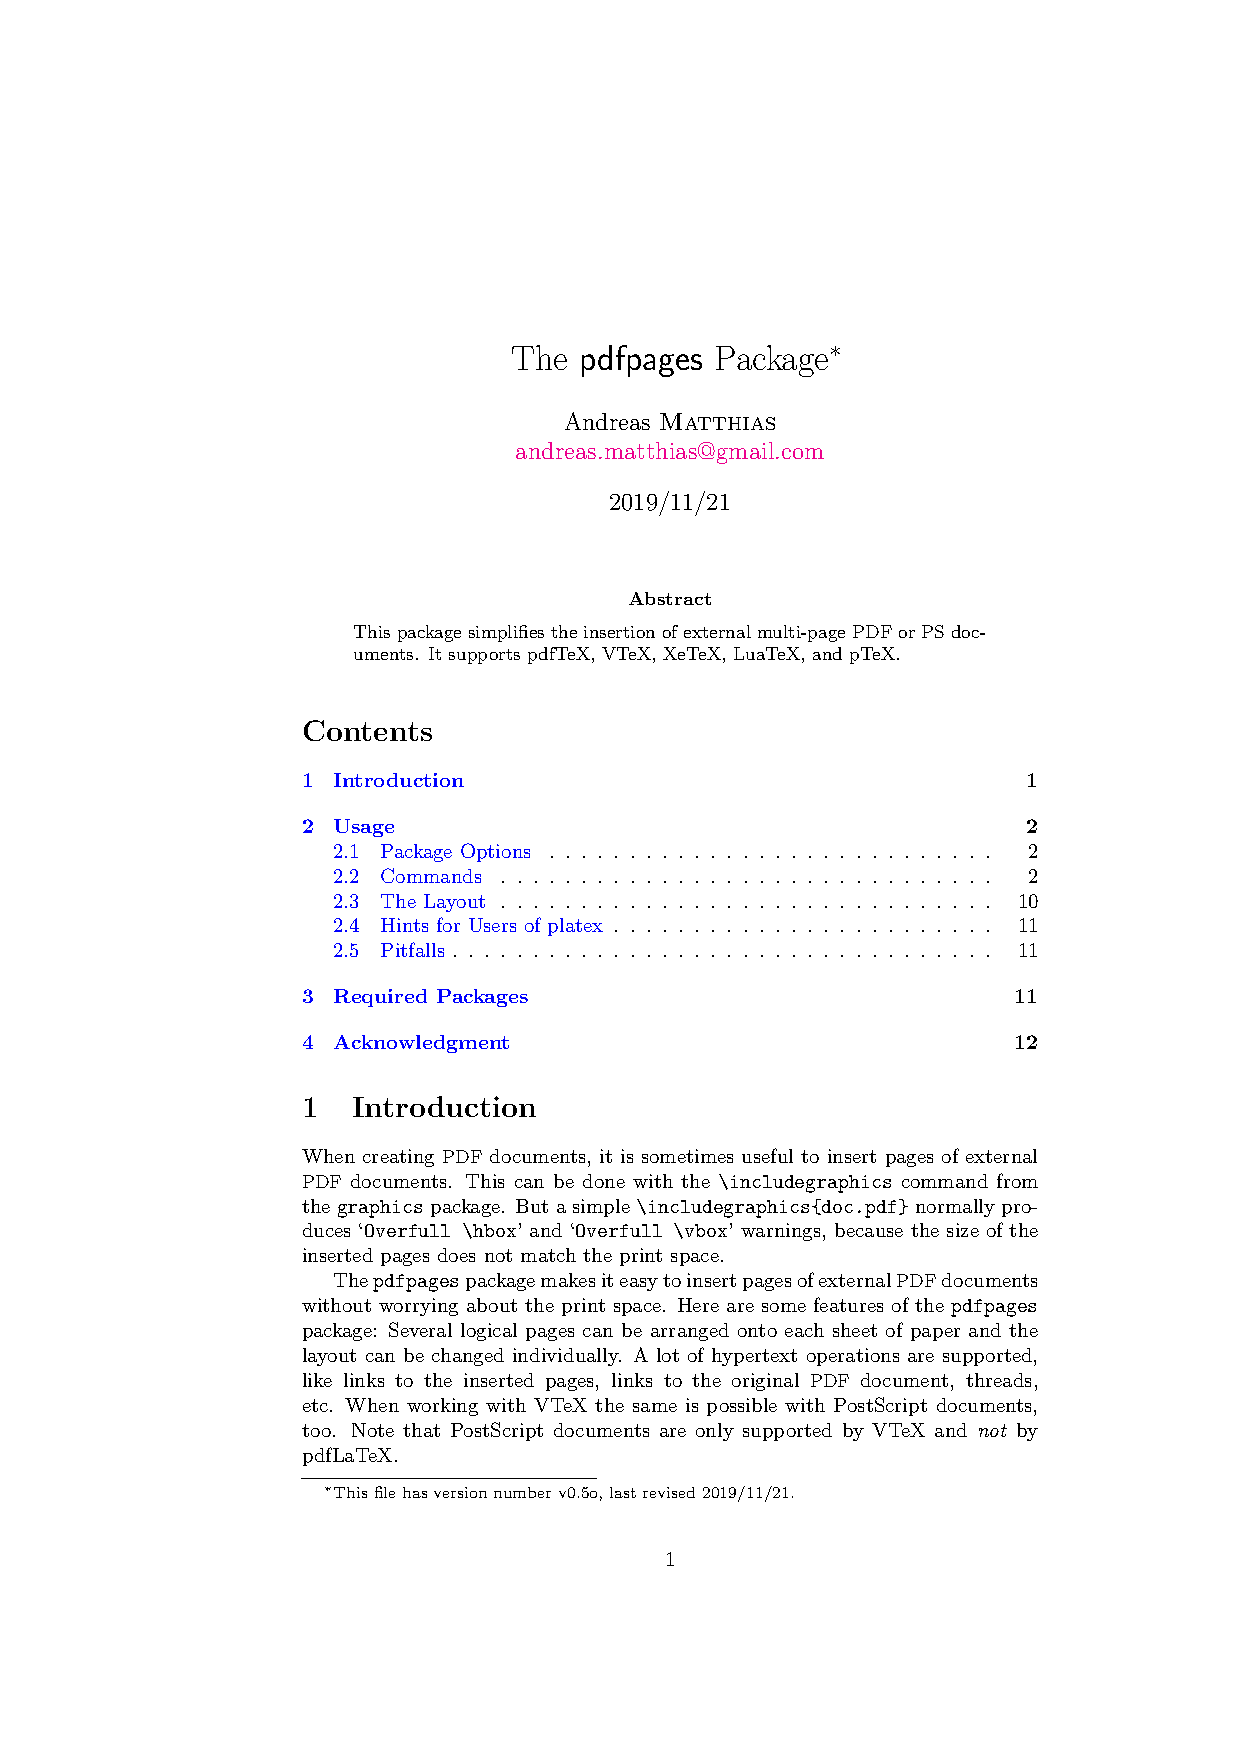
\includepdf[pages={1,3-5}]{PosTextuais/includepdfpages.pdf}
%\phantompart  \printindex  % Indice Remissivo
% ----------------------------------------------------------
\end{document}  % fim do documento
